\documentclass[UTF8,a4paper,11pt,fontset=fandol]{ctexart}
\usepackage[margin=23mm,headheight=15pt]{geometry}
\usepackage{amsmath,amssymb,bm,booktabs,tabularx,longtable,array,graphicx}
\usepackage{xcolor,fancyhdr,enumitem,caption,xurl}
\usepackage{tikz}
\usetikzlibrary{arrows.meta,positioning}
\usepackage[numbers,sort&compress]{natbib}
\usepackage[colorlinks=true,linkcolor=teal,citecolor=teal,urlcolor=teal,bookmarksnumbered=true]{hyperref}
\definecolor{ink}{HTML}{16324F}
\ctexset{section={format=\Large\bfseries\color{ink}},subsection={format=\large\bfseries}}
\AddToHook{cmd/section/before}{\clearpage}
\pagestyle{fancy}\fancyhf{}
\fancyhead[L]{\small 牵引引导与全身柔顺控制}
\fancyhead[R]{\small 代码分析与研究方案}
\fancyfoot[C]{\thepage}
\setlength{\parskip}{4pt}
\setlist{nosep,leftmargin=2em}
\renewcommand{\arraystretch}{1.22}
\newcolumntype{P}[1]{>{\raggedright\arraybackslash}p{#1}}
\newcolumntype{Y}{>{\raggedright\arraybackslash}X}
\newcommand{\R}{\mathbb{R}}
\newcommand{\clip}{\operatorname{clip}}
\newcommand{\sgn}{\operatorname{sign}}
\newcommand{\code}[1]{\texttt{\nolinkurl{#1}}}
\newcommand{\ev}[1]{\textsuperscript{[代码 #1]}}
\hypersetup{pdftitle={牵引引导与全身柔顺控制：当前实现分析、相关方法与评价协议},pdfauthor={zhanghao0625}}
\title{\vspace{-12mm}\textbf{牵引引导与全身柔顺控制}\\[5pt]\Large 当前实现分析、相关方法与评价协议}
\author{旧版 H6 基线与纯牵引方案的技术分析}
\date{2026 年 11 月 13 日}
\begin{document}
\maketitle
\begin{abstract}
本文研究外部速度指令为零时，四足机器人在牵引下的柔顺跟随与撤力停稳。旧版 H6 基线训练时对采样的速度指令叠加学习到的修正，平移参考修正一旦越过力阈值便立即饱和。当前纯牵引方案在冻结的 Policy8 底座上估计机身线速度、外力与力矩，并依据可调质量--阻尼参考训练策略直接生成速度指令。本文分析旧版基线的局限，说明纯牵引方案的网络、训练和部署方式，并按现有评分代码给出牵引响应、转正、速度跟随和停稳的评估协议。
\end{abstract}
\noindent\textbf{审阅范围}\quad 第~\ref{sec:h6-baseline} 至第~\ref{sec:h6-analysis} 节依据 \code{cts-moe-him} 的提交
\code{57a05ee00d229da6fd6f10defcc51e947247d6c6}，分析 H6 牵引 5k 实验的 \code{policy8_frozen_cts_teacher_aligned_v3} 基线。第~\ref{sec:evaluation} 和第~\ref{sec:pure-traction} 节依据 \code{vbot} 的 \code{dev1-pure-traction} 分支，提交为 \code{1810875}。文中的动力学曲线为公式计算结果，评估协议依据代码检查整理。
\clearpage
\tableofcontents
\newpage

\section{问题定义}
\subsection{复杂地形下的人机牵引柔顺运动控制}

人通过机器人手腕、把手或机身施加牵引力$F^s$，引导机器人平稳移动与转向，并在持续牵引下自适应通过复杂地形、保持动态平衡；牵引解除后，机器人平滑恢复原始速度指令。

\subsection{网络输入与输出}
每帧观测为 45 维，按以下顺序拼接：
\begin{equation}
\bm o_t=\left[
\bm c_t^{\rm obs},\;
\bm\omega_t^{\rm b},\;
\bm g_t^{\rm b},\;
(\bm q_t-\bm q_{\rm nom}),\;
\dot{\bm q}_t,\;
\bm a_{t-1}
\right]^\top\in\R^{45}.
\label{eq:proprio-observation}
\end{equation}
六项依次为速度指令（3）、机身角速度（3）、重力投影（3）、相对关节位置（12）、关节速度（12）和上一次关节动作（12）。其中 $\bm c_t^{\rm obs}$ 为观测中的速度指令。最近 $H$ 帧组成网络输入
\begin{equation}
h_t=\left[\bm o_t,\;\bm o_{t-1},\;\ldots,\;\bm o_{t-H+1}\right]^\top\in\R^{45H}.
\label{eq:proprio-history}
\end{equation}
两套方案均使用 $H=6$。前向、侧向和偏航是速度接口的三个分量。
旧版 H6 的网络输出速度修正，纯牵引策略直接输出速度指令。
各自的网络输入和反馈时序见第~\ref{sec:h6-baseline} 和第~\ref{sec:pure-traction} 节。

\subsection{速度指令与牵引力转换}

速度指令的平移分量采用 $\mathrm{m/s}$，偏航分量采用 $\mathrm{rad/s}$。

牵引力作用于点 $P$ 时，将力转换到机身坐标系 $b$，并计算关于机身参考点的等效力矩。
\begin{equation}
\bm F^b=\bm R_{bs}\bm F^s,
\qquad \bm\tau_{\rm eq}^b=\bm r_{bP}^b\times\bm F^b.
\label{eq:force-transform}
\end{equation}
其中 $\bm R_{bs}$ 将 $s$ 系向量旋转到 $b$ 系，$\bm r_{bP}^b$ 是机身参考点指向 $P$ 的位矢，以 $b$ 系表示。


\section{参考代码中的当前方案}

\begin{itemize}
  \item \textbf{网络结构}\enspace H6 牵引训练在冻结的运动控制模型上增加速度修正 MLP。
  \item \textbf{网络输出}\enspace MLP 根据本体观测、历史特征和指令反馈，每帧直接输出前向、侧向和偏航速度修正的均值。训练将处理后的修正叠加到下一帧的原始指令。\ev{C2,C4}
  \item \textbf{训练参考}\enspace 平移参考修正在各轴的力分量越过阈值后立即饱和，偏航参考随拉力方向变化。奖励以速度修正误差为目标，未规定加速度或起步过渡曲线。\ev{C5,C6}
  \item \textbf{撤力响应}\enspace 撤力使参考修正归零，奖励鼓励 MLP 消除残余修正。原始指令也为零时，期望机器人停车。当前训练缺少显式停车约束。\ev{C5,C6,C7}
  \item \textbf{部署指令}\enspace H6 v2 优先采用摇杆或 Follow 外部指令。外部指令幅值连续 $0.4\,\mathrm{s}$ 低于 $0.1$ 后，切换到 C++ 后处理后的网络速度输出。\href{https://github.com/VitaDynamics/cerebrix/blob/57a05ee00d229da6fd6f10defcc51e947247d6c6/source/cerebrix/cerebrix/rl/traction/contracts/deployment_h6_v2/deployment_contract.json\#L57}{部署契约}
\end{itemize}

本节对应 \code{--teacher_aligned} 的基线配方与 \code{source_v1} 采样。训练入口为 \code{train_frozen_latent.py}。\ev{C1,C3}

\subsection{网络设计}

训练时的网络结构与反馈见图~\ref{fig:h6-network-feedback}。观测沿用式~\eqref{eq:proprio-observation} 和式~\eqref{eq:proprio-history}，
取 $H=6$，关节动作项使用上一控制步的平滑动作。仿真机身线速度和力标签用于奖励与 Critic。\ev{C2,C4,C6}

\begin{itemize}
  \item 前向、侧向、偏航修正的限幅依次为 $[-0.5,1.3]$、$[-0.5,0.5]$、$[-1.5,1.5]$。
  \item 平移与偏航绝对值的死区阈值分别为 $0.05\,\mathrm{m/s}$ 和 $0.05\,\mathrm{rad/s}$。
  \item 导出网络的 \code{action_cmd} 为修正均值，后处理在网络外执行。\ev{C2,C3,C5}
\end{itemize}

令缩放系数 $S=\operatorname{diag}(2,2,0.25)$，常规控制帧的指令输入满足\ev{C4}
\begin{equation}
 o_t[0{:}3]=S(\bm c^0_t+\bm\delta_{t-1}),\qquad
 \mathrm{cmd\_ori}_t=[S\bm c^0_t,\ S\bm\delta_{t-1}].
\label{eq:redundant}
\end{equation}

\begin{figure}[!htbp]
\centering
\begin{tikzpicture}[
  node distance=5mm,
  block/.style={draw=ink,fill=ink!4,rounded corners=2pt,
    text width=116mm,minimum height=11mm,align=center,
    inner sep=5pt,font=\small},
  input/.style={block,text width=43mm,minimum height=17mm},
  >={Stealth[length=2mm]},line width=0.7pt
]
\node[input] (obs) at (-52mm,0) {\textbf{最新帧观测}\\[2pt]
  $\bm o_t$（45 维）};
\node[input] (latent) at (0,0) {\textbf{CTS 历史特征}\\[2pt]
  $\bm z_t$（32 维）};
\node[input] (cmd) at (52mm,0) {\textbf{指令反馈}\\[2pt]
  \texttt{cmd\_ori}（6 维）};

\node[block,below=9mm of latent] (mlp) {\textbf{速度修正 MLP}\quad $83\to256\to128\to3$};
\node[block,below=of mlp] (process) {\textbf{修正处理与反馈}\\[2pt]
  修正均值 $\bm\mu_t$（3 维，前向、侧向、偏航）\\[2pt]
  训练时从均值对应的分布采样，经限幅与死区得到 $\bm\delta_t$\\[2pt]
  将 $\bm\delta_t$ 写入下一帧指令反馈与观测
  \quad $\bm c^{\rm obs}_{t+1}=S(\bm c^0_{t+1}+\bm\delta_t)$};
\node[block,below=of process] (base) {\textbf{冻结运动控制模型}\\[2pt]
  输入 $h_{t+1}$，输出 12 维关节动作 $\bm a_{t+1}$};

\draw[->] (obs.south) -- ++(0,-4mm) -| ([xshift=-35mm]mlp.north);
\draw[->] (latent.south) -- (mlp.north);
\draw[->] (cmd.south) -- ++(0,-4mm) -| ([xshift=35mm]mlp.north);
\draw[->] (mlp) -- (process);
\draw[->] (process) -- (base);
\end{tikzpicture}

\caption{H6 速度修正网络的输入、输出与下一帧反馈。}
\label{fig:h6-network-feedback}
\end{figure}

\clearpage
\subsection{训练环境与采样}

\noindent\textbf{外力采样与施加}\ev{C7}
\begin{itemize}
  \item \textbf{采样范围}\enspace 在机身坐标系均匀采样 $F_x,F_y\in[-50,50]\,\mathrm N$、$F_z\in[-10,10]\,\mathrm N$。
  \item \textbf{周期时序}\enspace 各环境每隔 $4\,\mathrm{s}$ 同步独立采样，前 $3.02\,\mathrm{s}$ 保留采样值，后 $0.98\,\mathrm{s}$ 清零。
  \item \textbf{施力方式}\enspace 保留采样值期间，每隔 $0.02\,\mathrm{s}$ 向机身 \code{base} 刚体质心施力一次，每次持续 $0.005\,\mathrm{s}$，附加力矩为零。
  \item \textbf{奖励用力}\enspace 计算参考速度修正时使用采样幅值。
\end{itemize}

\noindent\textbf{原始速度指令采样}\ev{C1,C3,C7}
\begin{itemize}
  \item \textbf{采样时机}\enspace \code{traction/commands.py} 在环境重置时及回合内每隔 $10\,\mathrm{s}$ 重采平移指令和目标航向。
  \item \textbf{平移指令}\enspace 前向速度由地形课程采样，侧向速度在 $[-0.3,0.3]\,\mathrm{m/s}$ 内均匀抽取。平移指令范数不超过 $0.1\,\mathrm{m/s}$ 时，两轴清零。
  \item \textbf{偏航指令}\enspace 通常每隔 $0.02\,\mathrm{s}$ 根据航向误差更新。
  \item \textbf{撤力后}\enspace 原始速度指令继续按上述时序更新。
\end{itemize}

\noindent\textbf{地形与动力学随机化}\ev{C1}
\begin{itemize}
  \item \textbf{地形}\enspace 沿用运动任务的粗糙地形课程。
  \item \textbf{动力学}\enspace 沿用地面摩擦、载荷与质心等随机化设置。
\end{itemize}

\subsection{由外力计算参考速度修正}

取机身坐标系下的水平力 $\bm F_{xy}=(F_x,F_y)$。平移参考速度修正通过下式计算
\begin{equation}
 g(F;l,u)=\begin{cases}
 0,& |F|\le\alpha,\\
 \clip\left(\dfrac{F+\alpha\sgn(F)}{\beta},l,u\right),&|F|>\alpha,
 \end{cases}
 \qquad
 \begin{aligned}
 \delta_{x,\rm ref}&=g(F_x;-0.5,1.2),\\
 \delta_{y,\rm ref}&=g(F_y;-0.5,0.5).
 \end{aligned}
\label{eq:force-map}
\end{equation}
基线取 $\alpha=17.5\,\mathrm N$、$\beta=20\,\mathrm{N\,s/m}$。代码中的 $(F/\beta)(1+\alpha/|F|)$ 与式~\eqref{eq:force-map} 的非零分支等价。H6 \code{teacher_aligned} 基线将前向参考速度修正上限设为 $1.2\,\mathrm{m/s}$，原始配方的上限为 $1.0\,\mathrm{m/s}$。\ev{C3,C5}

偏航参考速度修正由力的方向角 $\theta=\operatorname{atan2}(F_y,F_x)$ 决定
\begin{equation}
 \delta_{\omega,\rm ref}=\begin{cases}
 \clip\left(\dfrac{\theta+0.6\sgn(\theta)}{2},-0.8,0.8\right),
 &\|\bm F_{xy}\|>17.5\,\mathrm N\ \text{且}\ |\theta|>0.6\,\mathrm{rad},\\
 0,&\text{其余情况}.
 \end{cases}
\end{equation}
参考速度修正按当前力标签逐步计算，力标签清零时参考速度修正随即归零。\ev{C3,C5,C7}

图~\ref{fig:force-reference-map} 直接调用 \code{source_force_to_velocity} 计算，并与原始奖励映射函数 \code{_get_force_to_vel} 逐点核对。平移分量越过 $17.5\,\mathrm N$ 阈值后立即饱和；偏航分量同时受水平力幅值和方向角控制。\ev{C3,C5}

\noindent\begin{minipage}{\linewidth}
\captionsetup{hypcap=false}
\centering
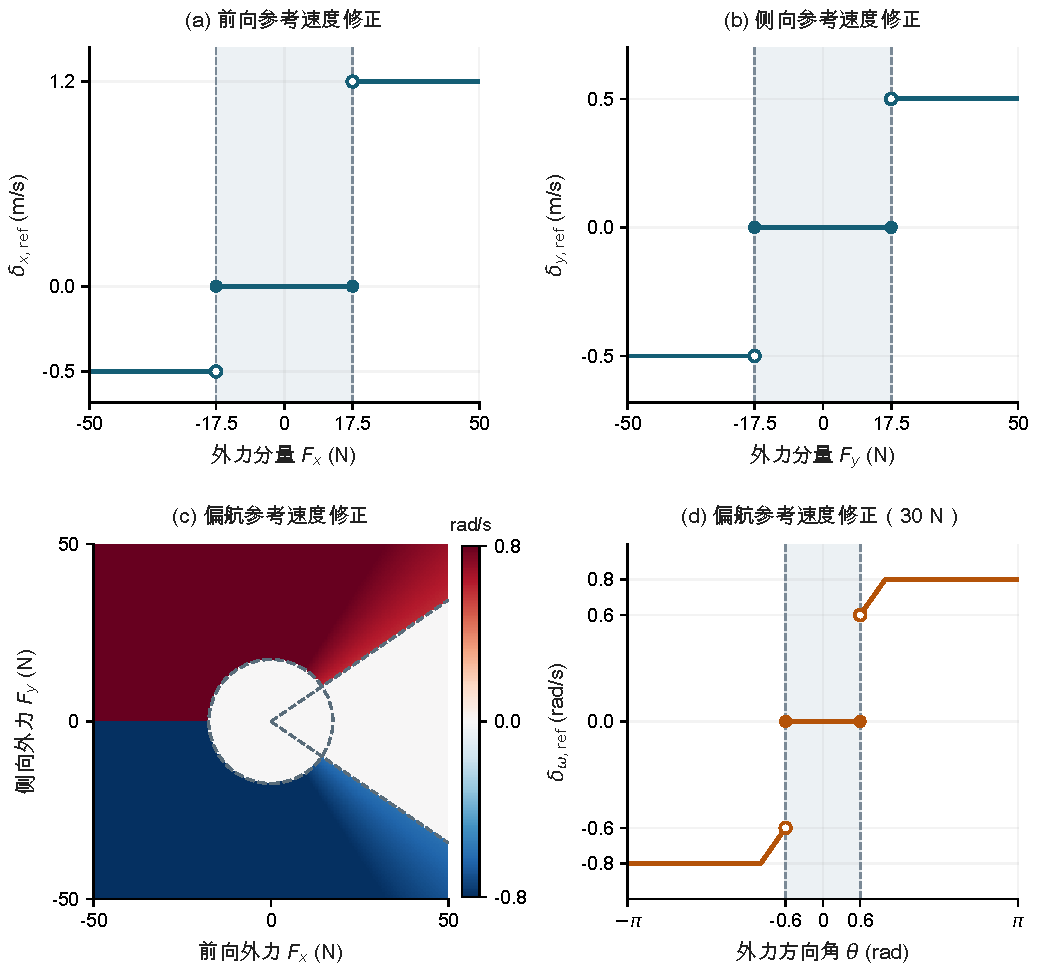
\includegraphics[width=0.84\linewidth]{figures/reference_map.pdf}
\captionof{figure}{外力与参考速度修正的关系。参数采用 H6 基线。子图 (a)、(b) 为前向、侧向映射；(c) 为偏航参考速度修正在水平力平面中的分布；(d) 为水平拉力大小固定为 $30\,\mathrm N$ 时，偏航参考速度修正随拉力方向的变化。实心点表示阈值处取值，空心点表示非零分支的极限，阴影表示死区。}
\label{fig:force-reference-map}
\end{minipage}\par

\subsection{奖励设计}

\noindent\textbf{牵引任务}\quad
\code{compliance} 比较本帧处理后的修正 $\bm\delta_t$ 与当前力标签生成的参考速度修正 $\bm\delta_{\rm ref,t}$。\ev{C6}
\begin{equation}
 r_{\rm comp,t}=-\|\bm\delta_{xy,t}-\bm\delta_{xy,\rm ref,t}\|^2
 -0.05(\delta_{\omega,t}-\delta_{\omega,\rm ref,t})^2.
\label{eq:comp}
\end{equation}

\noindent\textbf{运动跟踪}\quad
当前实现沿用底层运动跟踪奖励。跟踪目标为 $\bm c_{\rm trk,t}=\bm c^{0,\rm rew}_t+\bm\delta_{t-1}$，其中 $\bm c^{0,\rm rew}_t$ 是物理步结束后更新的原始指令，$\bm v_{xy,t}$ 和 $\omega_{z,t}$ 是此时的仿真机身速度。\ev{C6,C7}
\begin{align}
 r_{v,t}&=\exp\left(-\frac{\|\bm c_{\rm trk,xy,t}-\bm v_{xy,t}\|^2}{0.25}\right),&
 r_{\omega,t}&=\exp\left(-\frac{(c_{\rm trk,\omega,t}-\omega_{z,t})^2}{0.25}\right).
\end{align}
上述三项权重依次为 $5$、$1$、$0.5$，与其他奖励加权求和后乘控制步长。运动跟踪通过 PPO 回报影响牵引 MLP 学到的修正。物理步结束后更新力标签并计算奖励，新标签对应下一控制步排队施加的力。\ev{C6,C7,C8}

\noindent\textbf{稳定性与 PPO}\quad
其余奖励包含近零指令下的站姿、姿态、碰撞和关节动作平滑等。关节位置、力矩和速度限位作为三路约束代价。PPO 更新修正 MLP、采样标准差及奖励和代价 Critic，底座在牵引训练期间冻结。\ev{C6,C8}\cite{schulman2017}


\section{当前实现的问题分析}
\label{sec:h6-analysis}

本节分析第~\ref{sec:h6-baseline} 节所述的旧版 H6 基线。

\begin{enumerate}[itemsep=0.55em]
  \item \textbf{83 维输入中有 3 维可重建。}
  由式~\eqref{eq:redundant}，常规控制帧中，最新观测的前 3 维等于 \code{cmd_ori} 中两组三维向量的和。保留原始指令和上一帧修正，即可从 MLP 输入中省去合成指令三维。去冗余对训练性能的影响仍需消融验证。\ev{C2,C4}

  \item \textbf{仿真施力与头部附近牵引存在差异。}
  旧版仿真在质心施力。实际从头部附近牵引时，拉点相对质心的偏移会产生等效力矩，见式~\eqref{eq:force-transform}。此外，参考映射使用脉冲峰值，机器人只在控制周期的部分时间内受力。\ev{C7}

  \item \textbf{平移参考修正越过阈值就饱和。}
  式~\eqref{eq:force-map} 中，任一平移轴的力幅值刚超过 $17.5\,\mathrm{N}$，限幅前的修正幅值就已超过 $1.75\,\mathrm{m/s}$，直接达到该轴的限幅。例如，$18\,\mathrm{N}$ 和 $50\,\mathrm{N}$ 的前向力都对应 $1.2\,\mathrm{m/s}$ 的参考修正，阈值以上的力幅值差异无法反映到平移参考中。\ev{C3,C5}

  \item \textbf{运动跟踪奖励的设计与牵引任务不匹配。}
  底层负责跟踪给定速度，牵引 MLP 从观测中学习与外力对应的速度修正。当前平移和偏航跟踪奖励仍计入牵引 PPO 回报，而底层已冻结。其跟踪目标为原始指令加上一帧 MLP 修正，策略可能通过选取底层更容易执行的修正来提高跟踪分，即使该修正偏离外力参考。这两项跟踪奖励应留在底层控制训练中。\ev{C6,C8}

  \item \textbf{撤力后的实际减速过程与停车判据未明确。}
  旧版基线在撤力后将参考修正清零。纯牵引部署时外部原始指令为零，停车取决于网络输出是否回零，以及底座如何减速。第~\ref{sec:evaluation} 节依据撤力后的位移、航向、直立状态和底座执行指令评估停稳。\ev{C5,C6,C7,C11}

  \item \textbf{力标签比实际施力提前一帧。}
  当前控制步先用旧力完成仿真，再更新力标签，并用新标签计算本帧的 \code{compliance}。例如，撤力边界这一帧仍受最后一次非零力脉冲，奖励目标却已归零，到下一帧才停止施力。这是切换时相差一个控制步（$0.02\,\mathrm{s}$）的时序错误，基线因复现原实现而保留了这一行为。\ev{C6,C7,C8}
\end{enumerate}


\section{评价指标与实验协议}

论文对照采用 \code{vbot} 纯牵引平地仿真协议。每次试验静置 $4\,\mathrm{s}$，施力 $7\,\mathrm{s}$，撤力后观察 $5\,\mathrm{s}$，控制周期为 $0.02\,\mathrm{s}$。以施力前的机头为基准，分别在前、左、右、后四个方向施加 $10$ 或 $30\,\mathrm{N}$ 的恒定世界系水平力，共 8 个用例。结果按拉力大小分别汇总，通过率同时报告通过数和试验总数。

\subsection{关键指标}

$\uparrow$ 表示越大越好，$\downarrow$ 表示越小越好。

\subsubsection{2 秒内牵引响应通过率 \texorpdfstring{$\uparrow$}{↑}}
施力后 $2\,\mathrm{s}$ 内，实际沿力速度首次连续 $0.2\,\mathrm{s}$ 不低于 $0.10\,\mathrm{m/s}$，且施力后半段的平均沿力速度也不低于该阈值。

\subsubsection{转正通过率 \texorpdfstring{$\uparrow$}{↑}}
仅统计左、右、后拉。机头与拉力夹角须连续 $0.3\,\mathrm{s}$ 不超过 $15^\circ$，施力结束前的最后 $0.3\,\mathrm{s}$ 也须满足该条件。

\subsubsection{平面速度跟随 RMSE \texorpdfstring{$\downarrow$}{↓}}
在完整施力段，对齐控制步和机身坐标系，计算实际平面速度与质量--阻尼参考速度之间欧氏距离的均方根，单位为 $\mathrm{m/s}$。各方法使用相同的参考规则和参数。

\subsubsection{撤力后 3 秒内停稳率 \texorpdfstring{$\uparrow$}{↑}}
机器人须在撤力后 $3\,\mathrm{s}$ 内停稳，并保持至第 $5\,\mathrm{s}$。停稳后，每个 $1\,\mathrm{s}$ 窗口内的最大平面位移和航向变化分别不超过 $7\,\mathrm{cm}$ 和 $0.10\,\mathrm{rad}$，且保持直立、无重置。处理后的 MLP 执行指令还须满足平均平移幅值不超过 $0.05\,\mathrm{m/s}$、平均绝对偏航指令不超过 $0.10\,\mathrm{rad/s}$。

\subsubsection{撤力后 5 秒最大位移 \texorpdfstring{$\downarrow$}{↓}}
以撤力瞬间的位置为起点，取随后 $5\,\mathrm{s}$ 内的最大平面位移，单位为 $\mathrm{cm}$。

\subsection{其余指标}

\subsubsection{牵引响应时间 \texorpdfstring{$\downarrow$}{↓}}
从施力开始到首次满足持续沿力速度条件的时间。

\subsubsection{移动方向余弦 \texorpdfstring{$\uparrow$}{↑}}
计算施力后半段的平均实际平移速度与拉力方向的余弦，达到 $0.50$ 即通过。

\subsubsection{转正时间 \texorpdfstring{$\downarrow$}{↓}}
从施力开始到首次满足持续朝向条件的时间，并记录施力前后的朝向误差。

\subsubsection{转正后沿力速度}
取首次转正后 $0.5$--$2\,\mathrm{s}$ 的平均实际沿力速度，并检查窗口内是否保持对准。

\subsubsection{相对正拉速度比（接近 1 为佳）}
将转正后的平均沿力速度除以同档正拉在同一施力时段的平均沿力速度。正拉速度低于 $0.10\,\mathrm{m/s}$ 时省略该比例。

\subsubsection{撤力后停稳时间 \texorpdfstring{$\downarrow$}{↓}}
从撤力到首次满足停车判据并能持续稳定至观察结束的时间。

\subsubsection{撤力末段站稳率 \texorpdfstring{$\uparrow$}{↑}}
撤力后最后 $1\,\mathrm{s}$ 内，最大平面位移不超过 $5\,\mathrm{cm}$，航向变化不超过 $0.10\,\mathrm{rad}$，且保持直立、无重置。

\subsubsection{全程直立率 \texorpdfstring{$\uparrow$}{↑}}
逐例记录直立帧占比，汇总全程每帧均直立的试验数和比例。该项独立报告。

\subsubsection{全程无重置}
检查试验期间是否发生回合重置。

\subsubsection{撤力综合通过率 \texorpdfstring{$\uparrow$}{↑}}
统计同时满足按时停稳、末段站稳及全程无重置的试验比例。

\subsubsection{总通过率 \texorpdfstring{$\uparrow$}{↑}}
统计通过所有适用行为判据的试验比例。

\subsubsection{执行指令跟踪 RMSE \texorpdfstring{$\downarrow$}{↓}}
按前向、侧向和偏航分别计算实际速度相对底层执行指令的 RMSE。

\subsubsection{状态估计 RMSE \texorpdfstring{$\downarrow$}{↓}}
比较估计值与仿真真值，报告速度、外力和外力矩的 RMSE，并单列转正窗口内的前向力 RMSE。

\subsubsection{转正后指令均值}
在转正窗口内分别记录参考指令、MLP 原始输出和底层执行指令的均值。


\clearpage
\section{相关工作与可迁移方法}
\subsection{相关论文与适用范围}
\begin{table}[htbp]\centering\small
\begin{tabularx}{\linewidth}{P{32mm}Y Y}
\toprule 文献 & 主要机制 & 对当前问题的参考价值\\\midrule
FACET，2025\cite{facet2025} & 虚拟质量--弹簧--阻尼参考，teacher--student，GRU & 可调动力学响应与隐状态估计\\
Seeing-Eye Quadruped，2023\cite{defazio2023} & 监督学习估计外力，RL 保持行走，牵引指导导航 & 分开评估外力感知与运动执行\\
Learning Force Control，2024\cite{portela2024} & 末端力跟踪 RL，历史观测估计特权状态 & 机械臂与腿的全身力控制\\
Safe Whole-Body Loco-Manipulation，2026\cite{schperberg2026} & 腕部 F/T、显式导纳、腿部 RL、Reference Governor & 有力传感器时的模块化实现\\
Residual RL，2018 预印本\cite{johannink2018} & 已有控制器与学习残差叠加 & 明确残差的作用层级与职责\\\bottomrule
\end{tabularx}
\caption{选取的相近原始研究。年份采用参考文献中列出的版本。平台、传感器和任务差异应随对比实验一起记录。}
\end{table}

\subsection{FACET 的动态参考与 teacher--student}
FACET 用虚拟动力学生成 CoM 参考轨迹，其核心形式为
\begin{equation}
 m\ddot{\bm x}_{\rm ref}=K_p(\bm x_{\rm des}-\bm x_{\rm ref})
 +K_d(\dot{\bm x}_{\rm des}-\dot{\bm x}_{\rm ref})+\bm f_{\rm ext}.
\end{equation}
策略通过位置与速度跟踪奖励学习响应，并在多个时间起点生成的参考之间进行平滑。第一阶段用特权信息训练 teacher，同时用历史传感信息训练估计器预测特权特征。第二阶段以 teacher 初始化 student，并继续用 PPO 适应估计误差。论文中的估计器为隐藏维度 256 的 GRU，策略输出关节目标。该方法提供动态参考、参数条件化与隐状态估计的组合。\cite{facet2025}

第~\ref{sec:pure-traction} 节将虚拟动力学用于生成速度参考，由冻结底座执行速度指令。闭环跟随仍受底座运动能力和响应时延限制。

\subsection{监督力估计与直接全身力控制}
Seeing-Eye 方法同时训练本体观测驱动的速度与外力估计器和 RL 行走策略。估计器使用仿真真值监督，估计力方向用于生成导航目标。本文同样用仿真真值监督估计器，第~\ref{sec:evaluation} 节分别定义估计误差和底座执行误差。\cite{defazio2023}

Portela 等的方法把末端力命令直接纳入任务，策略协调机械臂与腿。历史观测估计模块用监督损失学习特权状态，actor/critic 用 PPO 训练，奖励包含末端力、位置和机身运动项。该结构适合进一步扩展手腕交互，机器人模型、输出动作和训练环境都需支持机械臂。\cite{portela2024}

\subsection{显式导纳与运动 RL 的组合}
Schperberg 等使用腕部六维 F/T 传感器，将外部力旋量映射为末端速度，由机械臂与腿共同跟踪。其 Reference Governor 根据模型约束调整参考，状态估计采用神经网络增强的 Kalman filter。论文展示了 Go2 与六自由度机械臂上的交互。其约束保证依赖模型和假设，迁移时需重新建立对应的约束集合。\cite{schperberg2026}

对于配备力传感器的系统，可用测力结果与导纳模型生成底座速度指令。若采用学习残差进一步补偿，可将修正写为
\begin{equation}
 \bm\delta_t=\bm\delta_{\rm adm,t}+\bm r_\theta(h_t,\bm c^0_t,\bm\delta_{\rm adm,t}),
\end{equation}
其中 $\bm r_\theta$ 有幅值约束，用于补偿底座跟踪误差和地形影响。这是将 Residual RL 迁移到速度指令层的一种设计。\cite{johannink2018}

\subsection{质量--阻尼参考的离散化示例}
考虑理想单轴质量--阻尼模型 $m\dot\delta+d\delta=F$，其中 $\delta$ 是参考速度。若周期内 $F$ 恒定，精确离散化为
\begin{equation}
 \delta_{k+1}=e^{-d\Delta t/m}\delta_k+
 \frac{1-e^{-d\Delta t/m}}{d}F_k.
\label{eq:exact}
\end{equation}
取 $m=10\,\mathrm{kg}$、$d=20\,\mathrm{N\,s/m}$、$\Delta t=0.02\,\mathrm s$。理想模型在恒定 $20\,\mathrm N$ 正拉下趋于 $1\,\mathrm{m/s}$，起步首个控制步约为 $0.0392\,\mathrm{m/s}$，撤力后每步乘以 $e^{-0.04}$。第~\ref{sec:pure-traction} 节在离散更新中加入力阈值与状态清零规则。同样的正拉场景下，纯牵引参考的稳态值为 $0.75\,\mathrm{m/s}$。

\begin{figure}[!htbp]\centering
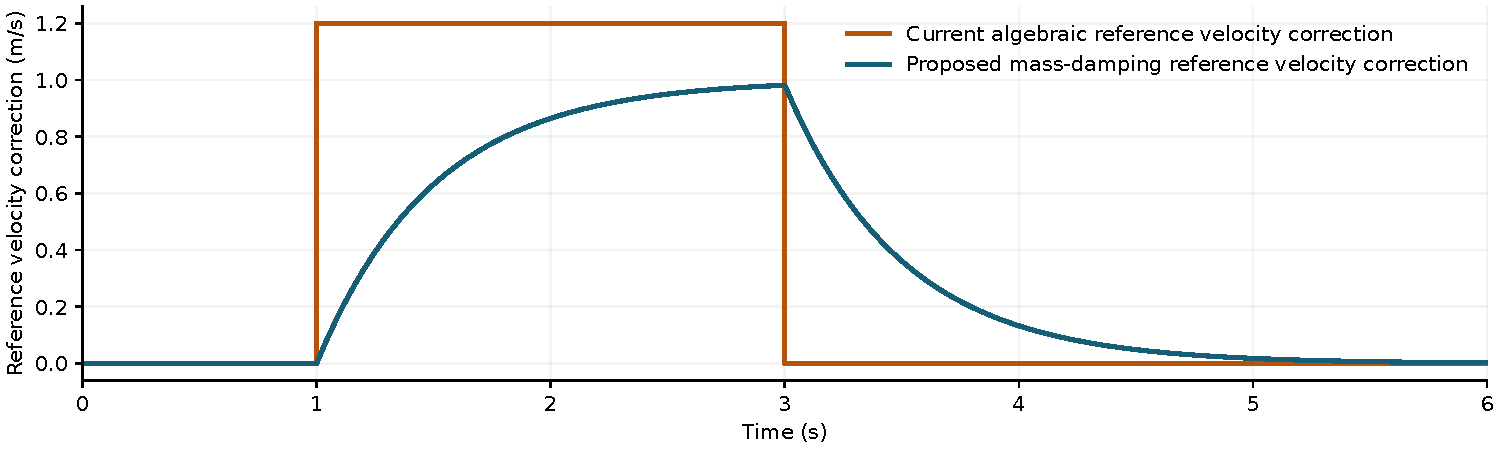
\includegraphics[width=\linewidth]{figures/reference_dynamics.pdf}
\caption{旧版 H6 基线与无力阈值、无状态清零的理想质量--阻尼模型。$1\le t<3\,\mathrm s$ 时施加 $20\,\mathrm N$ 正拉，其余时间为零。曲线均为参考量的计算结果。}
\end{figure}

后续可在统一参考和相同数据预算下，对比速度策略的监督模仿与 PPO，并比较直接测力、本体观测监督估计及循环网络估计。完整关节级 teacher--student 与冻结底座方案分别报告结果。


\section{我们的方法}
\label{sec:pure-traction}

本节对应 \code{vbot} 的 \code{dev1-pure-traction} 分支，提交为 \code{1810875}。纯牵引方案训练状态估计器和速度策略，直接生成前向、侧向和偏航速度指令。\ev{C14}

\subsection{网络设计}
网络层宽与反馈路径见图~\ref{fig:pure-traction-network}。
\begin{itemize}
  \item \textbf{状态估计器}\enspace 用最近 6 帧本体观测（270 维）估计机身线速度、外力和力矩（归一化，各 3 维）。
  \item \textbf{速度策略}\enspace 最新观测、估计量与 $(D,\tau)$ 组成 $45+9+2=56$ 维输入。参数归一化至 $[-1,1]$，估计量截断梯度。
  \item \textbf{策略原始输出}\enspace 训练时从对角高斯分布采样 $\bm u_t$，评估与部署时取均值。
  \item \textbf{指令后处理}\enspace $\mathcal P$ 先按前向 $[-0.5,1.3]$、侧向 $[-0.5,0.5]$（$\mathrm{m/s}$）和偏航 $[-1.5,1.5]$（$\mathrm{rad/s}$）限幅。平移范数 $\le 0.05\,\mathrm{m/s}$ 或偏航绝对值 $\le 0.05\,\mathrm{rad/s}$ 时清零对应分量。
  \item \textbf{下一帧反馈}\enspace Policy8 使用当前观测中的 $\bm c_t$。本步输出 $\bm c_{t+1}=\mathcal P(\bm u_t)$ 按图中的 $S$ 缩放后写入下一帧。
\end{itemize}

\begin{figure}[!htbp]
\centering
\begin{tikzpicture}[
  block/.style={draw=ink,fill=ink!4,rounded corners=2pt,
    align=center,inner sep=4pt,font=\small},
  input/.style={block,minimum height=19mm},
  estimate output/.style={block,text width=12mm,minimum height=8mm,
    inner sep=1.4pt,font=\footnotesize},
  >={Stealth[length=2mm]},line width=0.7pt
]
\node[block,text width=73mm,minimum height=14mm] (history) at (-16mm,0)
  {\textbf{本体观测历史}\quad $h_t$（6 帧，270 维）\\[2pt]
   最新帧含缩放后的当前执行指令 $S\bm c_t$};

\node[input,text width=28mm] (base) at (-58mm,-25mm)
  {\textbf{冻结 Policy8}\\[2pt]关节动作 $\bm a_t$\\（12 维）};
\node[input,text width=36mm] (estimate) at (-17mm,-25mm)
  {\textbf{状态估计器}\\[2pt]
   \mbox{\scriptsize $270\!\to\!512\!\to\!256\!\to\!128\!\to\!9$}\\[2pt]
   {\footnotesize 归一化输出（9 维）}};
\node[input,text width=27mm] (latest) at (23mm,-25mm)
  {\textbf{最新帧观测}\\[2pt]$\bm o_t$（45 维）};
\node[input,text width=27mm] (parameters) at (61mm,-25mm)
  {\textbf{参考参数}\\[2pt]$(D,\tau)$ 归一化\\（2 维）};

\node[estimate output] (velocity) at (-33mm,-42.5mm) {线速度\\3 维};
\node[estimate output] (force) at (-17mm,-42.5mm) {外力\\3 维};
\node[estimate output] (moment) at (-1mm,-42.5mm) {力矩\\3 维};

\node[block,text width=28mm,minimum height=17mm] (simulation) at (-58mm,-60mm)
  {\textbf{仿真执行}\\[2pt]获取下一帧本体状态};
\node[block,fill=ink!8,text width=96mm,minimum height=15mm] (actor) at (23mm,-60mm)
  {\textbf{速度策略 MLP}\quad $56\to256\to128\to64\to3$\\[2pt]
   输出前向、侧向、偏航速度均值};
\node[block,text width=96mm,minimum height=15mm] (process) at (23mm,-80mm)
  {\textbf{限幅与死区}\\[2pt]
   训练时采样，推理时取均值，再处理原始指令 $\bm u_t$\\[2pt]
   $\bm c_{t+1}=\mathcal P(\bm u_t)$};
\node[block,text width=128mm,minimum height=14mm] (next) at (-4mm,-106mm)
  {\textbf{更新下一帧观测}\quad
   $\bm o_{t+1}[0{:}3]=S\bm c_{t+1}$，$S=\operatorname{diag}(2,2,0.25)$\\[2pt]
   将新观测加入历史 $h_{t+1}$};

\draw[->] ([xshift=-30mm]history.south) -- ++(0,-4mm) -| (base.north);
\draw[->] ([xshift=-1mm]history.south) -- (estimate.north);
\draw[->] ([xshift=29mm]history.south) -- ++(0,-4mm) -| (latest.north);
\draw[->] (base.south) -- (simulation.north);
\coordinate (estimate-split) at (-17mm,-36.5mm);
\draw (estimate.south) -- (estimate-split);
\draw[->] (estimate-split) -| (velocity.north);
\draw[->] (estimate-split) -- (force.north);
\draw[->] (estimate-split) -| (moment.north);
\coordinate (estimate-merge) at (-17mm,-48.8mm);
\draw (velocity.south) |- (estimate-merge);
\draw (force.south) -- (estimate-merge);
\draw (moment.south) |- (estimate-merge);
\draw[->] (estimate-merge) -- node[right,font=\scriptsize] {截断梯度} ([xshift=-40mm]actor.north);
\draw[->] (latest.south) -- (actor.north);
\draw[->] (parameters.south) -- ([xshift=38mm]actor.north);
\draw[->] (actor.south) -- (process.north);
\draw[->] (simulation.south) -- ([xshift=-54mm]next.north);
\draw[->] (process.south) -- ([xshift=27mm]next.north);
\coordinate (loop) at (79mm,0);
\draw[->,dashed,draw=ink!65] (next.east) -- (loop |- next.east) -- (loop)
  -- node[above,font=\footnotesize] {进入下一控制步} (history.east);
\end{tikzpicture}

\caption{网络架构}
\label{fig:pure-traction-network}
\end{figure}

\subsection{训练环境与采样}
\begin{itemize}
  \item \textbf{训练环境}\enspace 在 Vita01evt 粗糙地形仿真中训练，冻结 Policy8 运动底座，控制周期为 $0.02\,\mathrm{s}$。
  \item \textbf{回合类别}\enspace 按 $25\%$ 无力、$25\%$ 弱力、$50\%$ 常规牵引分配回合。无力回合全程施力为零。
  \item \textbf{施力时序}\enspace 弱力和常规牵引回合默认每 $10\,\mathrm{s}$ 重采一次世界系外力，保持 $7\,\mathrm{s}$，再清零 $3\,\mathrm{s}$。
  \item \textbf{弱力采样}\enspace 幅值均匀采自 $[0,10)\,\mathrm N$，方向在单位球面均匀采样。
  \item \textbf{常规牵引采样}\enspace 三个世界系力分量独立均匀采自 $[-40,40)\,\mathrm N$。
  \item \textbf{施力方式}\enspace 作用点 $\bm r^b$ 在机身原点前方 $0.17287\,\mathrm m$。按式~\eqref{eq:force-transform} 将外力转为机身系 $\bm F_t^b$，在质心施加该力和力矩 $(\bm r^b-\bm r_{\rm CoM}^b)\times\bm F_t^b$。其中 $\bm r_{\rm CoM}^b$ 为机身原点至质心的向量。\ev{C12}
  \item \textbf{监督标签}\enspace 使用机身系线速度、外力 $\bm F_t^b$ 和关于机身原点的力矩 $\bm r^b\times\bm F_t^b$。力标签和参考速度均由生成当前观测的控制段所施加的外力更新。
\end{itemize}

\subsection{由外力计算参考速度}

\subsubsection{质量--弹簧--阻尼模型}
设 $x$ 为参考位移，$x_0$ 为平衡位置。单轴虚拟质量--弹簧--阻尼模型在外力 $F$ 下满足
\begin{equation}
 M\ddot x+D\dot x+K(x-x_0)=F.
\end{equation}
\begin{itemize}
  \item \textbf{弹簧刚度 $K$}\enspace 产生指向平衡位置的恢复力。$K,D>0$ 时，恒力使位移 $x-x_0$ 趋于 $F/K$。
  \item \textbf{虚拟质量 $M$}\enspace 同一净力下，质量越大，加速度越小。从平衡位置静止起步时，初始加速度为 $F/M$。
  \item \textbf{阻尼 $D$}\enspace 产生与速度方向相反的力，耗散运动能量并使响应趋于稳定。
\end{itemize}

\subsubsection{平移参考速度}
\label{subsec:planar-reference}
纯牵引取 $K=0$，取消位置恢复力。令 $v=\dot x$，则 $M\dot v+Dv=F$。恒定有效拉力下，限幅前的参考速度趋于 $F/D$，时间常数为 $\tau=M/D$。两个平移轴共用 $D$ 和 $M=D\tau$。训练时按回合独立均匀采样 $D\in[15,30]\,\mathrm{N\,s/m}$ 和 $\tau\in[0.3,0.8]\,\mathrm s$。标准评估默认取 $D=20\,\mathrm{N\,s/m}$、$\tau=0.5\,\mathrm s$，对应 $M=10\,\mathrm{kg}$。\ev{C11,C15}

令 $\rho_t=\|\bm F_t^w\|_2$、$F_0=5\,\mathrm N$，以施加的三维外力幅值判定力阈值。有效平移力为
\begin{equation}
 \bm F^{b}_{xy,\mathrm{eff},t}
 = \left(1-\frac{F_0}{\max(\rho_t,F_0)}\right)\bm F^{b}_{xy,t}.
\end{equation}
\begin{samepage}
更新前，先将上一控制步的内部平面速度 $\bm s_{t-1}$ 转到当前航向。设 $\psi_t$ 为机身航向，$R(\cdot)$ 为二维旋转矩阵，$a=e^{-\Delta t/\tau}$，控制周期 $\Delta t=0.02\,\mathrm s$。力幅值低于阈值时清零内部状态，其余情况按式~\eqref{eq:exact} 做零阶保持离散更新
\begin{equation}
 \bm s_t=
 \begin{cases}
 aR(\psi_{t-1}-\psi_t)\bm s_{t-1}+(1-a)\bm F^{b}_{xy,\mathrm{eff},t}/D,
   & \rho_t\ge F_0,\\
 \bm 0, & \rho_t<F_0.
 \end{cases}
\end{equation}
\end{samepage}

\begin{samepage}
\subsubsection{偏航参考速度}
三维合力与机身系水平力均达到 $5\,\mathrm N$ 时启用偏航参考。水平力方向角为 $\theta_t=\operatorname{atan2}(F^b_{y,t},F^b_{x,t})$。默认偏航增益 $0.5\,\mathrm{s}^{-1}$ 乘以有符号的转向角误差，得到限幅前的偏航速度 $\omega^{*}_{z,t}$。通常选最短转向。当 $|\theta_t|\ge170^\circ$ 且已有转向选择时沿用该方向，必要时按 $2\pi-|\theta_t|$ 计算转角。最后用 $\mathcal P$ 处理平移与偏航，得到参考指令 $\bm c_{{\rm ref},t}$。图~\ref{fig:traction-reference-map} 给出稳态示例。\ev{C15}
\par
\end{samepage}

\begin{figure}[!htbp]
\centering
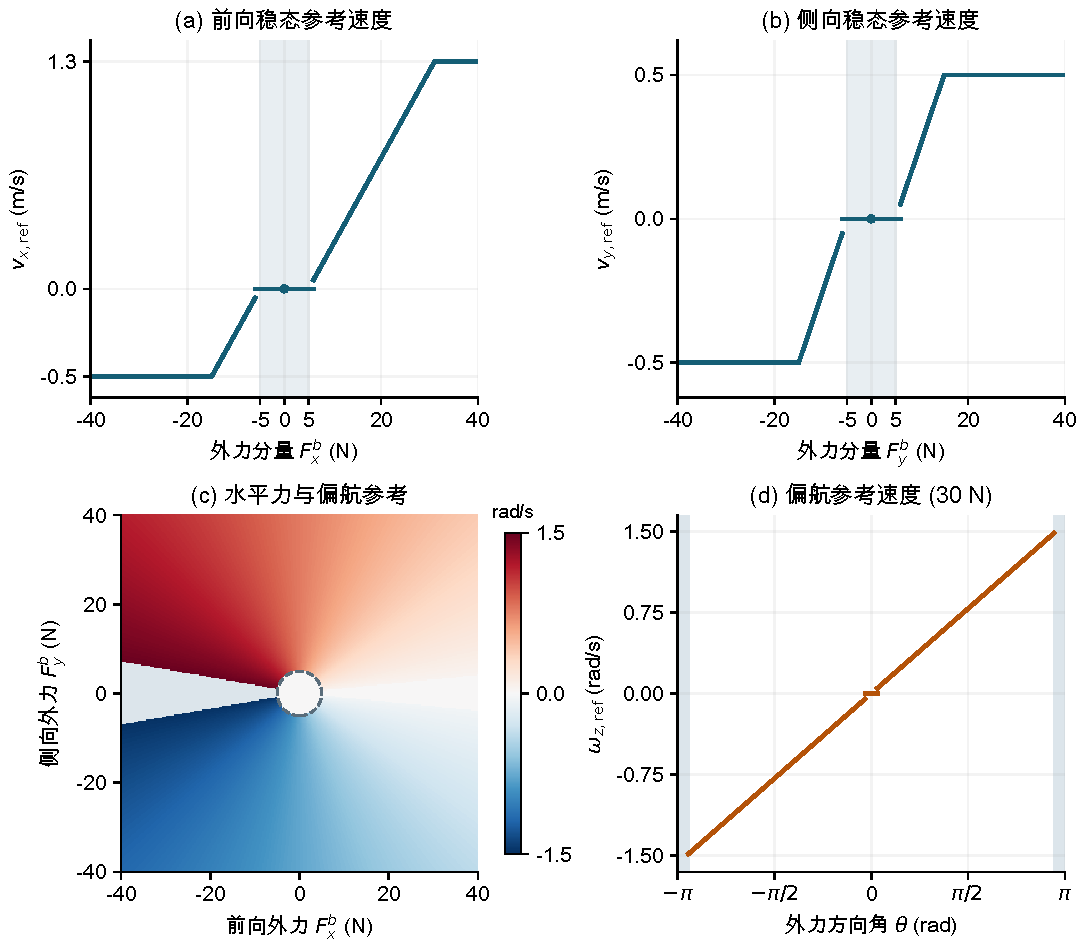
\includegraphics[width=0.76\linewidth]{figures/traction_reference_map.pdf}
\caption{纯牵引方案的外力与参考速度关系。取 $F_z^b=0$，$D=20\,\mathrm{N\,s/m}$。(a)、(b) 为单轴恒定施力时经后处理的稳态平移参考，(c)、(d) 为偏航参考的水平力分布和 $30\,\mathrm N$ 切片。后方灰区表示转向方向取决于历史选择。}
\label{fig:traction-reference-map}
\end{figure}

\begin{samepage}
\subsection{奖励设计}
令 $g_t=\mathbf 1_{\{\rho_t\ge F_0\}}$ 为当前观测对应的牵引标记，$\bm e_t=\bm u_t-\bm c_{{\rm ref},t}$ 为策略原始输出与参考指令的误差，$\bm d_t=\bm v_t-\bm c_t$ 为步末实际机身速度对本步执行指令的误差。下标 $xy$ 和 $\omega$ 分别表示平移与偏航，$\tilde{\bm a}_t$ 为平滑后的关节动作。单步奖励为 $\Delta t\sum_i w_i r_{i,t}$，各项 $r_{i,t}$ 见表~\ref{tab:pure-traction-rewards}。\ev{C12,C13}

\par\nobreak\medskip\noindent
\begin{minipage}{\linewidth}
\captionsetup{hypcap=false}
\small
\begin{tabularx}{\linewidth}{@{}P{48mm}Y>{\centering\arraybackslash}p{19mm}@{}}
\toprule
\textbf{奖励名称} & \textbf{计算方式} & \textbf{默认权重} \\
\midrule
\code{compliance_yaw} & $g_t\exp(-e_{\omega,t}^2)$ & $1$ \\
\code{compliance_lin_vel} & $g_t\exp(-\|\bm e_{xy,t}\|_2^2)$ & $2$ \\
\code{zero_command_lin_vel} & $(1-g_t)\|\bm u_{xy,t}\|_2^2$ & $-8$ \\
\code{zero_command_yaw} & $(1-g_t)u_{\omega,t}^2$ & $-4$ \\
\code{tracking_lin_vel} & $\exp(-\|\bm d_{xy,t}\|_2^2/0.25)$ & $1$ \\
\code{tracking_ang_vel} & $\exp(-d_{\omega,t}^2/0.25)$ & $0.5$ \\
\code{action_rate} & $\|\tilde{\bm a}_t-\tilde{\bm a}_{t-1}\|_2^2$ & $-0.01$ \\
\code{smoothness} & $\|\tilde{\bm a}_t-2\tilde{\bm a}_{t-1}+\tilde{\bm a}_{t-2}\|_2^2$ & $-0.01$ \\
\code{mlp_action_rate} & $\|\bm u_t-\bm u_{t-1}\|_2^2$ & $-0.01$ \\
\bottomrule
\end{tabularx}
\captionof{table}{纯牵引训练奖励项}
\label{tab:pure-traction-rewards}
\end{minipage}
\par
\end{samepage}

训练默认使用 4096 个环境，每轮采集 24 个控制步。先用带约束代价的 PPO 更新速度策略与价值网络，再用同一批轨迹的观测和仿真标签更新估计器。PPO 的折扣系数、GAE 系数和裁剪幅度分别为 $0.99$、$0.95$ 和 $0.2$。估计损失对线速度、外力和力矩分别计算归一化 MSE 后加权求和。三组标签尺度为 $(1,40,7)$，权重默认为 $(1,1,1)$。两套 Adam 优化器的默认学习率均为 $10^{-3}$。

\subsection{评估与部署接口}
仿真评估模式见第~\ref{sec:evaluation} 节。部署用的 ONNX 接收 270 维观测历史和物理单位下的 $(D,\tau)$，输出 12 维关节动作、3 维策略速度均值 $\bm u_t$ 和恢复至物理单位的 9 维状态估计。控制侧按前述限幅、死区与缩放规则更新下一帧观测。\ev{C14}


\clearpage
\appendix
\section{代码证据索引与复核方式}
下列路径相对于各自的仓库根目录。旧版 H6 基线对应 \code{cts-moe-him} 的提交 \code{57a05ee00d229da6fd6f10defcc51e947247d6c6}，纯牵引方案对应 \code{vbot} 的提交 \code{1810875}。

\small
\begin{longtable}{P{9mm}P{96mm}P{37mm}}
\toprule 编号 & 路径与定位 & 支持的结论\\\midrule\endhead
\bottomrule\endlastfoot
\multicolumn{3}{l}{\textbf{旧版 H6 基线}}\\*
C1 & \code{source/cerebrix/cerebrix/tasks/manager_based/traction/config/rough_env_cfg.py}；\code{agents/traction_cfg.py}（相对 config 目录） & 环境继承、外力接管、基线策略类\\
C2 & \code{source/cerebrix/cerebrix/rl/traction/latent_adapter.py} 的 \code{FrozenLatentAdapter} 和 \code{command_mean}；\code{models.py} 的 \code{_mlp} & 83 维输入、层宽、ELU、critic\\
C3 & \code{source/cerebrix/cerebrix/rl/traction/teacher_aligned.py} 和 \code{latent_mechanisms.py} & $1.2$ 上限、初始化、采样开关\\
C4 & \code{source/cerebrix/cerebrix/rl/traction/isaac_adapter.py} 的 \code{_critic_obs}；\code{latent_isaac.py}；\code{deployment_contract.py}；\code{source/cerebrix/cerebrix/utils/wrappers/himloco/vecenv_wrapper.py} & 合成指令、缩放、观测顺序与反馈\\
C5 & \code{source/cerebrix/cerebrix/rl/traction/tensors.py} 的 \code{source_force_to_velocity}、\code{source_process_command}；\code{reference/reward_methods.py} 的 \code{_get_force_to_vel} & 参考速度修正计算与修正动作处理\\
C6 & \code{source/cerebrix/cerebrix/rl/traction/reference/reward_methods.py}；\code{reward_scales.json}、\code{source_recipe_parameters.json}（同目录）；\code{isaac_rewards.py} & reward 公式、权重与 dt\\
C7 & \code{source/cerebrix/cerebrix/rl/traction/source_force_v2.py}；\code{source_force_isaac_v2.py}；\code{control.py} & 质心施力、物理子步、标签更新\\
C8 & \code{source/cerebrix/cerebrix/rl/traction/latent_runner.py}；\code{latent_ppo.py}；\code{latent_feedback.py} & 交互时序、PPO、无独立估计器更新\\
C9 & \code{docs/experiments/vita01evt_go2_transfer/p13_h6_traction_5k_20261101.md} & H6 5k 配方与既有实验背景\\
C10 & \code{scripts/reinforcement_learning/traction/evaluate_frozen_latent.py}、\code{run_frozen_latent_long.py}（同目录）；\code{latent_pull_evaluation.py}、\code{latent_pose_evaluation.py}、\code{latent_evaluation.py}（相对 \code{rl/traction}） & 旧版基线评估\\
\midrule
\multicolumn{3}{l}{\textbf{当前纯牵引方案}}\\*
C11 & \code{scripts/reinforcement_learning/pure_traction/evaluate.py}；\code{source/cerebrix/cerebrix/rl/pure_traction/evaluation.py} 的 \code{score_pull}、\code{release_windows} 和 \code{following_metrics} & 标准协议、评估模式、评分和汇总\\
C12 & \code{source/cerebrix/cerebrix/tasks/manager_based/pure_traction/task.py}；\code{source/cerebrix/cerebrix/rl/pure_traction/force.py} & 施力点、标签时序、执行指令、直立判定\\
C13 & \code{source/cerebrix/cerebrix/tasks/manager_based/pure_traction/config.py}；\code{source/cerebrix/cerebrix/tasks/manager_based/locomotion/velocity/config/quadruped/vita_vita01evt/himloco_rewards.py} & 奖励项、默认权重、动作平滑\\
C14 & \code{source/cerebrix/cerebrix/rl/pure_traction/} 下的 \code{model.py}、\code{learner.py} 和 \code{runner.py} & 网络结构、参数更新、ONNX 导出\\
C15 & \code{source/cerebrix/cerebrix/rl/pure_traction/reference.py} & 力阈值、平移和偏航参考\\
\end{longtable}
\normalsize
旧版 H6 基线的代码提交入口为
\url{https://github.com/VitaDynamics/cerebrix/tree/57a05ee00d229da6fd6f10defcc51e947247d6c6}。

可用 \code{scripts/plot_reference.py} 重建旧版力映射和理想模型示意图，用 \code{scripts/plot_traction_reference.py} 重建纯牵引稳态参考图。


\begingroup
\raggedright
\bibliographystyle{plainnat}
\bibliography{references}
\endgroup
\end{document}
